%\newpage

\section{Full Example}
\label{sec:full-example}

\subsection{Non Serializable Counterexample}

\paragraph{Serializable NFA Extraction.}

Continuing the running (non-serializable) example presented in Listing~\ref{lst:MotivatingExample2NonSer}, the NS presented in Fig.~\ref{fig:code2ExampleNS} allows us to also extract the NFA encoding all serial executions. The states encode the global variable values, and the edges encode request/response pairs for all serial executions. As can be seen, serial executions can produce only pairs of the type ({\color{ForestGreen}$\blacklozenge_\text{main}$/{\color{red}$\blacklozenge_1$}}):

\begin{figure}[!htbp]
	\centering
	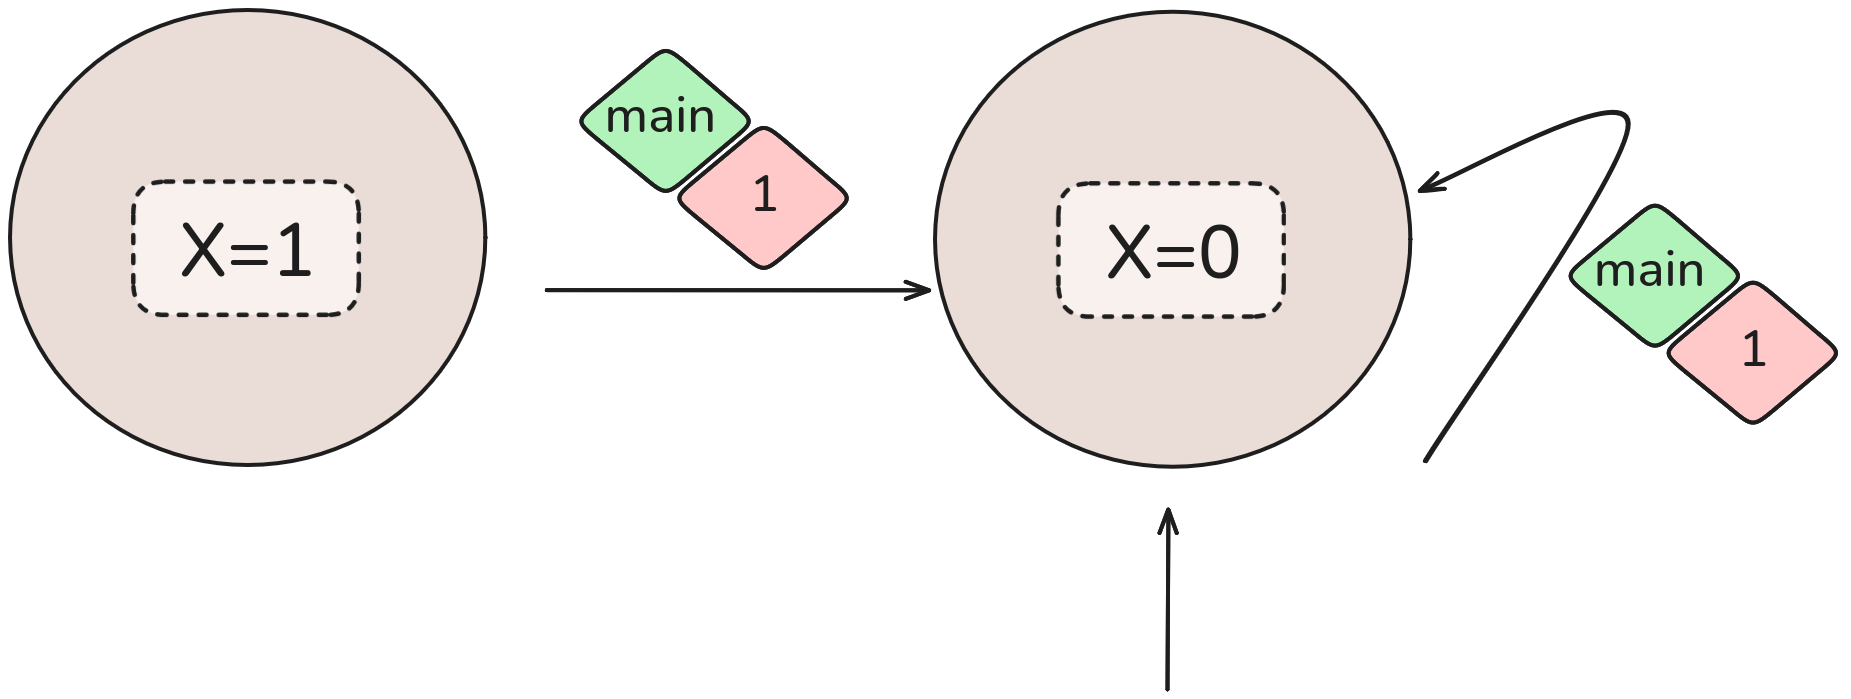
\includegraphics[width=0.5\textwidth,trim=0 0 0 0,clip]{plots/code_2_NFA.png}
	\caption{NFA for serialized executions of Listing~\ref{lst:MotivatingExample2NonSer} program.}
	\label{fig:code2ExampleNFA}
\end{figure}

\paragraph{Petri Net Extraction.}

Finally, the NS allows to generate the following Petri Net, encoding all possible interleavings of our program:

\begin{figure}[!htbp]
	\centering
	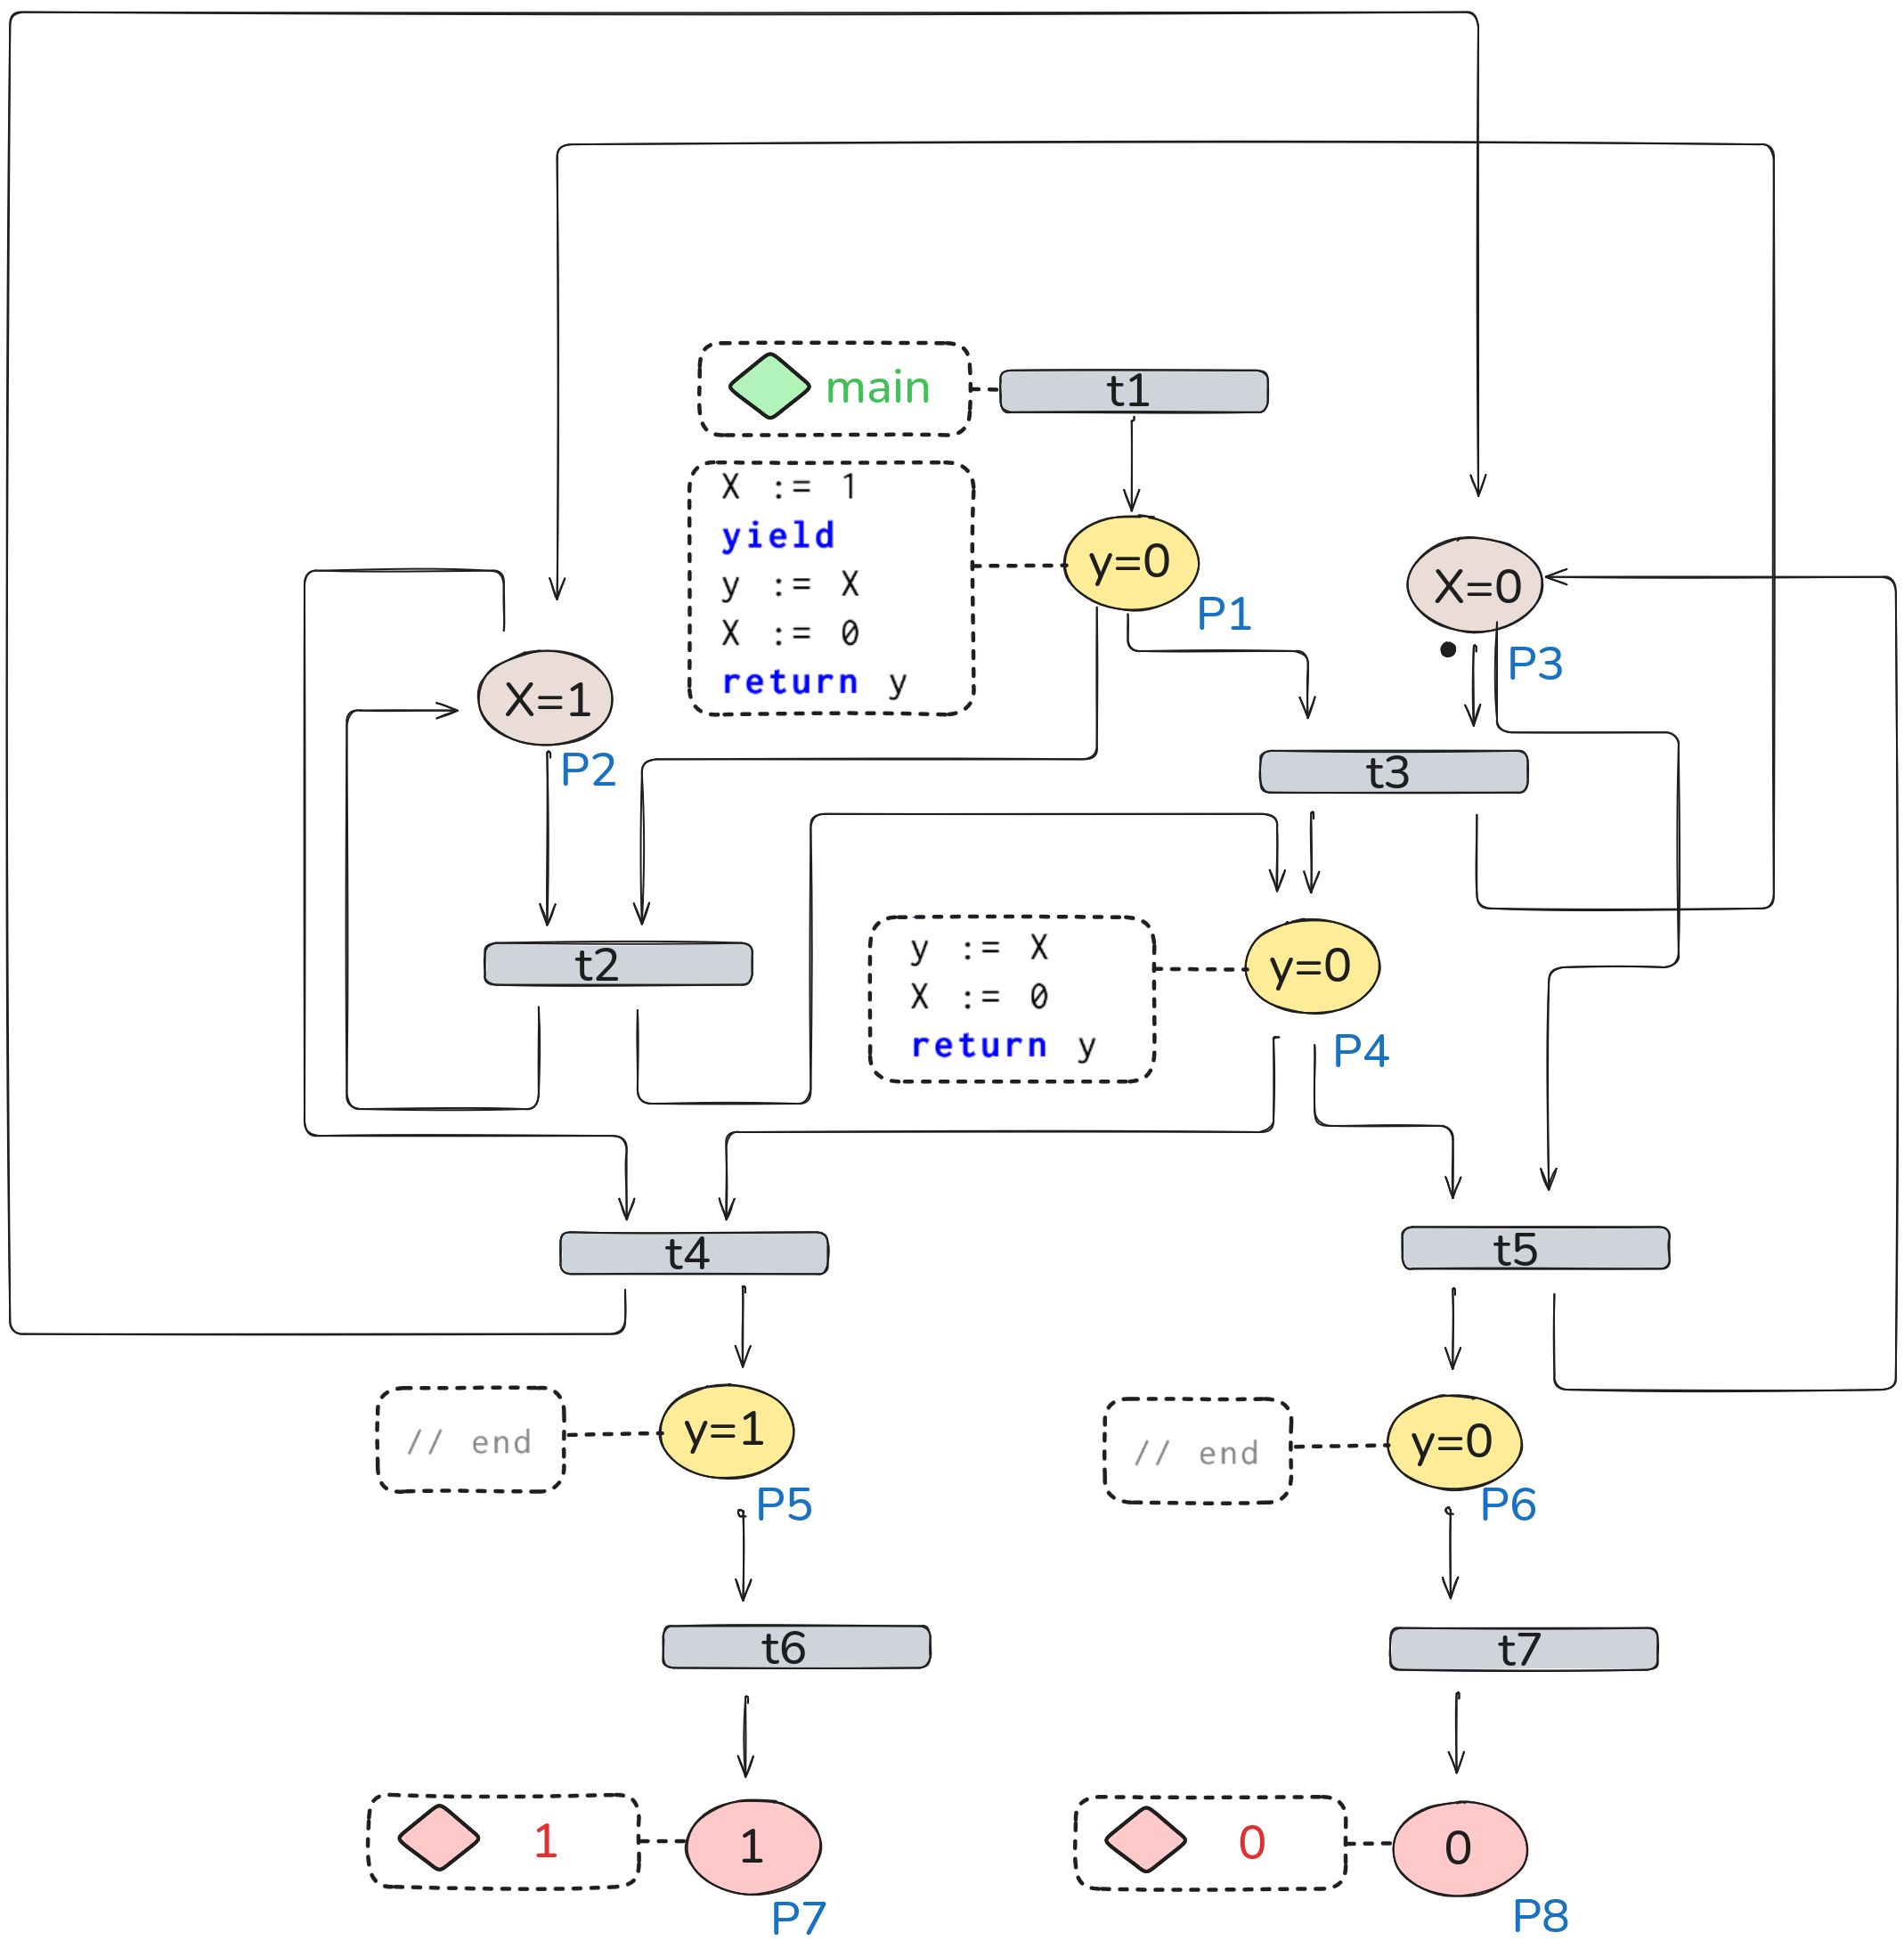
\includegraphics[width=0.7\textwidth]{plots/code_2_PN_with_annotation.png}
	\caption{Petri Net for interleaving executions of Listing~\ref{lst:MotivatingExample2NonSer} program. Note that there is no firing sequence that can reach the place representing a response of ``0'', i.e., the bottom right place.}
	\label{fig:code2ExamplePN}
\end{figure}

The places represent the $\delta$ transitions of our NS --- encoding either a ``step'' of our program, or spawning a request ($t_1$, which  corresponds to spawning request {\color{ForestGreen}$\blacklozenge_\text{main}$}), or returning a responds, e.g. transitions $t_6,t_7$ that corresponds to outputting responses {\color{red}$\blacklozenge_1$},{\color{red}$\blacklozenge_0$}.
%
Some places (\textcolor{blue}{$P_2$},\textcolor{blue}{$P_3$}) corresponds to the global state, while others ($P_1,P_4,P_5,P_6$) corresponds to the local state of an in-flight request.
%
Each token corresponds to a single packet, or (in the case of the global-variable-encoding places), to the global state of the program.

\paragraph{Counterexample Extraction.}

Regarding the aforementioned program, we automatically generate the following LTL reachability query for the Petri net of Figure~\ref{fig:code1ExamplePN} (which, if satisfiable, indicates the program is not serializable):

\todo{fix the "exists Marking M"}

\[
\exists\,M.\; 
P_1 = 0 \wedge 
\textcolor{blue}{P_2} \ge 0 \wedge \textcolor{blue}{P_3} \ge 0  \wedge P_4 = 0
\wedge P_5 = 0 \wedge P_6 = 0 \wedge \textcolor{red}{P_7} = 0 \wedge \textcolor{red}{P_8} \ge 1.
\]
This asserts the existence of a marking with no tokens on $P_1,P_4,P_5,P_6$, exactly zero tokens on $\textcolor{red}{P_7}$, at least one token on $\textcolor{red}{P_8}$, and arbitrary tokens on $\textcolor{blue}{P_2},\textcolor{blue}{P_3}$.  In fact, the target marking
\[
M^* = \{\textcolor{blue}{P_3}(1),\;\textcolor{red}{P_7}(1),\;\textcolor{red}{P_8}(1)\}
\]
is reachable.  Table~\ref{tab:PetriNetFiringCounterexample} lists a firing sequence that leads to $M^*$.





\begin{table}[H]
	\centering
	\label{tab:reach-seq}
	\begin{tabular}{c l c c c c c c}
		\toprule
		\textbf{Step} 
		& \textbf{Firing} 
		& \multicolumn{3}{c}{\textbf{Marking (after firing)}} 
		& \multicolumn{3}{c}{\textbf{Description (after firing)}} \\
		\cmidrule(lr){3-5} \cmidrule(lr){6-8}
		& 
		& \textbf{Global} 
		& \textbf{Local} 
		& \textbf{Responses} 
		& \textbf{Global state} 
		& \textbf{In-flight packets} 
		& \textbf{Responses} \\
		\midrule
		0 & --                                  
		& {\color{blue}$P_3$(1)}                  
		& --                                    
		& --                                    
		& {\color{blue}[X=0]}                   
		& --                          
		& --                                    \\
		1 & $t_1$ 
		& {\color{blue}$P_3$(1)}                  
		& $P_1$(1)                                
		& --                                    
		& {\color{blue}[X=0]}                   
		& {\color{ForestGreen}$\blacklozenge_\text{main}$} 
		& --                                    \\
		2 & $t_1$ 
		& {\color{blue}$P_3$(1)}                  
		& $P_1$(2)                                
		& --                                    
		& {\color{blue}[X=0]}                   
		& {\color{ForestGreen}$\blacklozenge_\text{main}$}, {\color{ForestGreen}$\blacklozenge_\text{main}$}  
		& --                                    \\
		3 & $t_3$                                  
		& {\color{blue}$P_2$(1)}                  
		& $P_1$(1),$P_4$(1)                          
		& --                                   
		&                                    {\color{blue}[X=1]}    
		&                                    {\color{black}$\blacklozenge_\text{until yield}$}, {\color{ForestGreen}$\blacklozenge_\text{main}$}   
		& --                                    \\
		4 & $t_2$                                  
		& {\color{blue}$P_2$(1)}                  
		& $P_4$(2)                                
		& --                                    
		&                                    {\color{blue}[X=1]}    
		&                                    {\color{black}$\blacklozenge_\text{until yield}$}, {\color{black}$\blacklozenge_\text{until yield}$}   
		& --                                    \\
		5 & $t_4$                                  
		& {\color{blue}$P_3$(1)}                  
		& $P_5$(1),$P_4$(1)                          
		& --                                    
		&                                   {\color{blue}[X=0]}     
		&                                    {\color{black}$\blacklozenge_\text{after yield}$}, {\color{black}$\blacklozenge_\text{until yield}$}   
		& --                                    \\
		6 & $t_6$                     
		& {\color{blue}$P_3$(1)}                  
		& $P_4$(1)                                
		& {\color{red}$P_7$(1)}                    
		&                                      	{\color{blue}[X=0]}  
		&                                    {\color{black}$\blacklozenge_\text{until yield}$}   
		&                                   {\color{red}$\blacklozenge_1$}     \\
		7 & $t_5$                                  
		& {\color{blue}$P_3$(1)}                  
		& $P_6$(1)                                
		& {\color{red}$P_7$(1)}                    
		&                                   {\color{blue}[X=0]}    
		&                                    {\color{black}$\blacklozenge_\text{after yield}$}      
		&                                   {\color{red}$\blacklozenge_1$}        \\
		8 & $t_7$                     
		& {\color{blue}$P_3$(1)}                                  
		& --                                    
		& {\color{red}$P_7$(1),\color{red}$P_8$(1)}    
		&                                   {\color{blue}[X=0]}    
		&                                   --    
		&                                   {\color{red}$\blacklozenge_0$}, {\color{red}$\blacklozenge_1$}       \\
		\bottomrule
	\end{tabular}
		\caption{Firing sequence reaching the target marking $M^*$. The marking $P_i(n_j)$ indicates that there are $n_j$ tokens on place $P_i$. The initial marking has a single token in the place encoding the initialized values of the global variables.}
		\label{tab:PetriNetFiringCounterexample}
\end{table}

%\newpage

\subsection{Serializability Proof Example}
\label{sec:ns-serializable}

Now, we observe again the adjusted program (as previously described in Listing~\ref{lst:MotivatingExample3Ser}):

We present the corresponding Network System, Serailizability NFA, and Interleaving Petri Net in Appendix~\ref{appendix:MoreNsExamples}.

Non-serializability corresponds to the above Petri Net being able to reach the following marking:

\[
\exists\,M.\; \textcolor{blue}
P_1 = 0 \wedge 
{P_2} \ge 0 \wedge \textcolor{blue}{P_3} \ge 0  \wedge P_4 = 0
\wedge P_5 = 0 \wedge P_6 = 0 \wedge \textcolor{red}{P_7} = 0 \wedge \textcolor{red}{P_8} \ge 1.
\]


Note that this happened to be the exact same property as encoding non-serializability in the previous example, however, the Petri Net places $(P_1,\ldots,P_8)$ encode different states that correspond to the updated program. For example, now each place in the PN that encodes a global state accounts for two global variables, $X$ and $L$. 
%
However, this semilinear encoding (of non serializability) is \textit{unreachable}, as witness by the following inductive invariant:


\[
\begin{aligned}
	&(P_{1},\textcolor{blue}{P_{2}},\textcolor{blue}{P_{3}},P_{4},P_{5},P_{6},\textcolor{red}{P_{7}},\textcolor{red}{P_{8}})
	\;\mapsto\;\\
	&\quad
	\exists\,e_{0},\dots,e_{5}\ge0.\;
	\Bigl(
	e_{2}-e_{1}+\textcolor{blue}{P_{3}}-1=0\;\land\;
	e_{2}+P_{1}-e_{5}=0\;\land\;
	P_{5}-e_{1}+e_{4}=0\;\land\\
	&\qquad\quad
	-\,e_{4}+\textcolor{red}{P_{7}}=0\;\land\;
	P_{6}+e_{3}-e_{0}=0\;\land\;
	\textcolor{red}{P_{8}}-e_{3}=0\;\land\\
	&\qquad\quad
	-\,e_{2}+e_{1}+e_{0}+P_{4}=0\;\land\;
	-\,e_{2}+e_{1}+\textcolor{blue}{P_{2}}=0
	\Bigr)
	\;\land\;
	\bigl(P_{4}-1\ge0\;\lor\;\textcolor{blue}{P_{3}}-1\ge0\bigr).
\end{aligned}
\]


We then revert this invariant to match our Network System, and project it to inputs/outputs of the system.
%
We get the following inductive invariants for each of the two global state:

\begin{proof}
	
	\medskip\noindent
	For global state \textcolor{blue}{[L=0,X=0]}
	the projected invariant is:
	\[
	\bigl(\,\text{\color{ForestGreen}$\blacklozenge_{\text{main}}$}/\text{\color{red}$\blacklozenge_{0}$},\;
	\text{\color{ForestGreen}$\blacklozenge_{\text{main}}$}/\text{\color{red}$\blacklozenge_{1}$}\bigr)
	\;\mapsto\;
	\exists\,e_{0},\dots,e_{5}\ge0.\;
	\begin{aligned}[t]
		& e_{2}-e_{1}=0,\quad
		e_{2}-e_{5}=0,\quad
		-e_{1}+e_{4}=0,\\
		& -e_{4}+\bigl(\text{\color{ForestGreen}$\blacklozenge_{\text{main}}$}/\text{\color{red}$\blacklozenge_{1}$}\bigr)=0,\quad
		-e_{0}+e_{3}=0,\quad
		-e_{3}+\bigl(\text{\color{ForestGreen}$\blacklozenge_{\text{main}}$}/\text{\color{red}$\blacklozenge_{0}$}\bigr)=0,\\
		& -e_{2}+e_{1}+e_{0}=0,\quad
		-e_{2}+e_{1}=0.
	\end{aligned}
	\]
	From these:
	\[
	e_{1}=e_{2}=e_{4}=e_{5}=(\;
	\text{\color{ForestGreen}$\blacklozenge_{\text{main}}$}/\text{\color{red}$\blacklozenge_{1}$}),\;
	e_{0}=e_{3}=
	(\text{\color{ForestGreen}$\blacklozenge_{\text{main}}$}/\text{\color{red}$\blacklozenge_{0}$}),
	\]
	and
	\[
	-e_{2}+e_{1}+e_{0}=0\;\Longrightarrow\;e_{0}=0.
	\]
	Thus
	\[
(	\text{\color{ForestGreen}$\blacklozenge_{\text{main}}$}/\text{\color{red}$\blacklozenge_{0}$})
	=0,
	\]
	so (\(\text{\color{ForestGreen}$\blacklozenge_{\text{main}}$}/\text{\color{red}$\blacklozenge_{0}$}\)) cannot be attained from the global state
	\textcolor{blue}{[L=0,X=0]}.
	
	\medskip\noindent
	Case 2: Global state \textcolor{blue}{[L=1,X=1]}.
	The projected invariant is:
	
	
	\[
	\bigl(\,\text{\color{ForestGreen}$\blacklozenge_{\text{main}}$}/\text{\color{red}$\blacklozenge_{0}$},\;
	\text{\color{ForestGreen}$\blacklozenge_{\text{main}}$}/\text{\color{red}$\blacklozenge_{1}$}\bigr)
	\;\mapsto\;
	\exists\,e_{0},\dots,e_{5}.\;\bot,
	\]
	which is unsatisfiable.  Hence, no completed‐request pair, and in particular no (\(\text{\color{ForestGreen}$\blacklozenge_{\text{main}}$}/\text{\color{red}$\blacklozenge_{0}$}\)) pair can occur in this state.
	
	\medskip\noindent
	\textbf{Conclusion.}
	In all reachable states
	it holds that there cannot be any request/response pairs of type
(	$	\text{\color{ForestGreen}$\blacklozenge_{\text{main}}$}/\text{\color{red}$\blacklozenge_{0}$}
	$).
	%
	Furthermore, this indicates that the only attainable request/response pairs are of the form 	($	\text{\color{ForestGreen}$\blacklozenge_{\text{main}}$}/\text{\color{red}$\blacklozenge_{1}$})
	$, which are in the language of of NFA for serial executions. Thus, this program is serializable.
	%
	We further show that these invariants are \textit{inductive}: they encompass the system’s initial state and, once satisfied, remain true for all subsequent executions.
\end{proof}



%\newpage